\documentclass[handout]{beamer}

\usetheme[progressbar=frametitle]{metropolis}
\usepackage{appendixnumberbeamer}
\usepackage{booktabs}
\usepackage{amsmath}
\usepackage{amssymb}
\usepackage{tcolorbox}
\definecolor{metropolisblue}{RGB}{39, 59, 94}



% Begin document
\begin{document}

% Title page
\title{Introduction}
\author{Nipun Batra}
\date{\today}
\institute{IIT Gandhinagar}
\maketitle

\begin{frame}{What}
    \begin{itemize}
        \item Predict with uncertainty
        \item Optimize any black box function
        \item Efficiently create a training set
        \item Generative modelling
    \end{itemize}

    
\end{frame}

\begin{frame}{Predict with Uncertainty: Classification}
    
\end{frame}

\begin{frame}{Predict with Uncertainty: Regression}
    
\end{frame}


\begin{frame}{Questions}
    \begin{itemize}
        \item We used squared error loss function for linear regression. Why?
        \item We used cross entropy loss function for logistic regression. Why?
        \item How does np.random.randn work?
        \item np.std(x) and pd.std(x) give different results. Why?

    \end{itemize}
    
\end{frame}

\begin{frame}{How: Bayes Rule}
    \begin{equation*}
        P(A|B) = \frac{P(B|A)P(A)}{P(B)}
    \end{equation*}
    
=    Rewriting it using the ML notation:
    \begin{equation*}
        \textcolor{blue}{P(\theta|D)} = \frac{\textcolor{green}{P(D|\theta)} \cdot \textcolor{red}{P(\theta)}}{\textcolor{purple}{P(D)}}
    \end{equation*}
    
    \begin{itemize}
        \item $\textcolor{blue}{P(\theta|D)}$ is called the posterior
        \item $\textcolor{green}{P(D|\theta)}$ is called the likelihood
        \item $\textcolor{red}{P(\theta)}$ is called the prior
        \item $\textcolor{purple}{P(D)}$ is called the evidence
    \end{itemize}
    
\end{frame}

\begin{frame}{Univariate Normal Distribution}
The probability density function of a univariate normal distribution is given by:

\begin{equation}
f(x|\mu, \sigma^2) = \frac{1}{\sqrt{2\pi\sigma^2}}\exp\left(-\frac{(x-\mu)^2}{2\sigma^2}\right)
\end{equation}

Let us assume we have a dataset $D = \{x_1, x_2, \ldots, x_n\}$, where each $x_i$ is an independent sample from the above distribution. 
We want to estimate the parameters $\theta = \{\mu, \sigma\}$ from the data.

Our likelihood function is given by:
\begin{equation}
P(D|\theta) = \mathcal{L}(\mu, \sigma^2) = \prod_{i=1}^n f(x_i|\mu, \sigma^2)
\end{equation}


\end{frame}

\begin{frame}{Log Likelihood Function}
    Log-likelihood function:
    \begin{equation}
        \log \mathcal{L}(\mu, \sigma^2) = \sum_{i=1}^n \log f(x_i|\mu, \sigma^2)
    \end{equation}

    Simplifying the above equation, we get:
    \begin{align*}
        \log \mathcal{L}(\mu, \sigma^2) &= \sum_{i=1}^n \log f(x_i|\mu, \sigma^2) \\
        &= \sum_{i=1}^n \log \left( \frac{1}{\sqrt{2\pi\sigma^2}} \exp \left( -\frac{(x_i-\mu)^2}{2\sigma^2} \right) \right) \\
        &= \sum_{i=1}^n \left( \log \left( \frac{1}{\sqrt{2\pi\sigma^2}} \right) + \log \left( \exp \left( -\frac{(x_i-\mu)^2}{2\sigma^2} \right) \right) \right) \\
        \end{align*}
\end{frame}

\begin{frame}
   
    \begin{align*}
        \log \mathcal{L}(\mu, \sigma^2) &= \sum_{i=1}^n \left( \log \left( \frac{1}{\sqrt{2\pi\sigma^2}} \right) -\frac{(x_i-\mu)^2}{2\sigma^2} \right) \\
        &= \sum_{i=1}^n \left( -\frac{1}{2} \log (2\pi\sigma^2) -\frac{(x_i-\mu)^2}{2\sigma^2} \right) \\
        &= -\frac{n}{2} \log (2\pi\sigma^2) - \frac{1}{2\sigma^2} \sum_{i=1}^n (x_i-\mu)^2
        \end{align*}
        \begin{tcolorbox}[colback=metropolisblue!5,colframe=metropolisblue,title=Log Likelihood Function for Univariate Normal Distribution]
            Log-likelihood function for normally distributed data is:
            \[
                \log \mathcal{L}(\mu, \sigma^2) = -\frac{n}{2} \log(2\pi) - n\log(\sigma) - \frac{1}{2\sigma^2} \sum_{i=1}^n (x_i-\mu)^2
                \]
        \end{tcolorbox}
\end{frame}








\begin{frame}
    \frametitle{Maximum Likelihood Estimate for $\mu$}
    
    To find the MLE for $\mu$, we differentiate the log-likelihood function with respect to $\mu$ and set it to zero:
    
    \begin{align*}
        \frac{\partial \log \mathcal{L}(\mu, \sigma^2)}{\partial \mu} &= \frac{\partial}{\partial \mu} \left(-\frac{n}{2} \log (2\pi\sigma^2) - \frac{1}{2\sigma^2} \sum_{i=1}^n (x_i-\mu)^2\right) =0\\
        \frac{\partial}{\partial \mu} \left(\sum_{i=1}^n (x_i-\mu)^2\right) &= 0
    \end{align*}
    
    \begin{tcolorbox}[colback=metropolisblue!5,colframe=metropolisblue,title=Maximum Likelihood Estimate for $\mu$]
        MLE of $\mu$, denoted as $\hat{\mu}_{\text{MLE}}$, is given by:
        \begin{equation*}
            \hat{\mu}_{\text{MLE}} = \frac{1}{n}\sum_{i=1}^n x_i
        \end{equation*}
    \end{tcolorbox}
    
    \end{frame}

\begin{frame}{MLE for $\sigma$ for normally distributed data}
    Recall that the log-likelihood function is given by:
    \begin{equation}
        \log \mathcal{L}(\mu, \sigma^2) = \sum_{i=1}^n \log f(x_i|\mu, \sigma^2)
    \end{equation}

    Let us find the maximum likelihood estimate of $\sigma^2$ now. We can do this by taking the derivative of the log-likelihood function with respect to $\sigma^2$ and equating it to zero.   

    \begin{equation}
        \frac{\partial \log \mathcal{L}(\mu, \sigma^2)}{\partial \sigma^2} = \sum_{i=1}^n \frac{\partial \log f(x_i|\mu, \sigma^2)}{\partial \sigma^2} = 0
    \end{equation}
    
\end{frame}

\begin{frame}{MLE for $\sigma$ for normally distributed data}
    \begin{tcolorbox}[colback=metropolisblue!5,colframe=metropolisblue,title=Log Likelihood Function for Univariate Normal Distribution]
        Log-likelihood function for normally distributed data is:
        \[
            \log \mathcal{L}(\mu, \sigma^2) = -\frac{n}{2} \log(2\pi) - n\log(\sigma) - \frac{1}{2\sigma^2} \sum_{i=1}^n (x_i-\mu)^2
            \]
    \end{tcolorbox}

Now, we can differentiate the log-likelihood function with respect to $\sigma$ and equate it to zero.
\end{frame}

\begin{frame}{MLE for $\sigma$ for normally distributed data}

    
        \[
        \frac{{\partial}}{{\partial \sigma}} \log \mathcal{L}(\mu, \sigma^2) = -\frac{n}{\sigma} + \frac{1}{\sigma^3} \sum_{i=1}^n (x_i-\mu)^2 = 0
        \]
    
        Multiplying through by $\sigma^3$, we have:
    
        \[
        -n \sigma^2 + \sum_{i=1}^n (x_i-\mu)^2 = 0
        \]
    
        \begin{tcolorbox}[colback=metropolisblue!5,colframe=metropolisblue,title=Maximum Likelihood Estimate for $\sigma^2$]
            MLE of $\sigma^2$, denoted as $\hat{\sigma}^2_{\text{MLE}}$, is given by:
            \[
                \sigma^2 = \frac{1}{n} \sum_{i=1}^n (x_i-\mu)^2
                \]
        \end{tcolorbox}
    
       

    \end{frame}
    

    \begin{frame}{Bias of an Estimator}
        \begin{tcolorbox}[colback=metropolisblue!5,colframe=metropolisblue,title=Bias of an Estimator]
            The bias of an estimator $\hat{\theta}$ of a parameter $\theta$ is defined as:
            \[
                \text{Bias}(\hat{\theta}) = \mathbb{E}(\hat{\theta}) - \theta
            \]
            where $\mathbb{E}(\hat{\theta})$ is the expected value of the estimator $\hat{\theta}$.
        \end{tcolorbox}
        \begin{itemize}
            \item An estimator is said to be unbiased if $\text{Bias}(\hat{\theta}) = 0$.
            \item An estimator is said to be biased if $\text{Bias}(\hat{\theta}) \neq 0$.
        \end{itemize}
        
    \end{frame}

    \begin{frame}{Bias of an Estimator: $\hat{\mu}_{MLE}$}
        \pause 
        Question: What is the expectation of $\hat{\mu}_{MLE}$ calculated over? What is the source of randomness?
        
        Let us assume that the true underlying distribution is $\mathcal{N}(\mu, \sigma^2)$.
    
        Let $\mathcal{D}^1 = \{x^1_1, x^1_2, \ldots, x^1_n\}$ be a dataset obtained from this distribution. 
    
        The MLE of $\mu$ based on $\mathcal{D}^1$ is given by:
        \begin{align*}
            \hat{\mu}_{MLE}^1 = \frac{1}{n} \sum_{i=1}^n x^1_i
        \end{align*}
    
        If we obtained another dataset $\mathcal{D}^2 = \{x^2_1,  x^2_2, \ldots, x^2_n\}$ from the same distribution, the MLE of $\mu$ based on $\mathcal{D}^2$ would be:
        \begin{align*}
            \hat{\mu}_{MLE}^2 = \frac{1}{n} \sum_{i=1}^n x^2_i
        \end{align*}
    \end{frame}
    
    \begin{frame}{Bias of an Estimator: $\hat{\mu}_{MLE}$}
        If we repeat this process and obtain datasets $\mathcal{D}^1, \mathcal{D}^2, \ldots, \mathcal{D}^k$, we would have $k$ different estimates of $\mu$.
    
        Taking the expectation of these $k$ estimates gives us the expected value of $\hat{\mu}_{MLE}$:
        \begin{align*}
            \mathbb{E}(\hat{\mu}_{MLE}) = \frac{1}{k} \sum_{i=1}^k \hat{\mu}_{MLE}^i
        \end{align*}
    
        Simplifying further, we have:
        \begin{align*}
            \mathbb{E}(\hat{\mu}_{MLE}) = \frac{1}{kn} \sum_{i=1}^k \sum_{j=1}^n x^i_j
        \end{align*}
        
        This expectation is calculated over multiple datasets $\mathcal{D}^1, \mathcal{D}^2, \ldots, \mathcal{D}^k$, where each dataset represents a different realization of the random variables from the underlying distribution.
        
       
    \end{frame}
    
    \begin{frame}{Bias of an Estimator: $\hat{\mu}_{MLE}$}
        To show that the estimator $\hat{\mu}_{MLE}$ is unbiased, we need to demonstrate that $\mathbb{E}(\hat{\mu}_{MLE}) = \mu$.
        
        Recall that each $x^i_j$ is a random variable following $\mathcal{N}(\mu, \sigma^2)$. Therefore, the sum $\sum_{i=1}^k x^i_j$ follows $\mathcal{N}(k\mu, k\sigma^2)$.
        
        Thus, we can write:
        \begin{align*}
            \mathbb{E}(\hat{\mu}_{MLE}) &= \frac{1}{kn} \sum_{i=1}^k \sum_{j=1}^n x^i_j = \frac{1}{kn} \sum_{j=1}^n \left(\sum_{i=1}^k x^i_j\right) \\
            &= \frac{1}{kn} \sum_{j=1}^n (k\mu) = \frac{1}{kn} (kn\mu) =\mu
        \end{align*}
        
        % Add tcolorbox here
        \begin{tcolorbox}[colback=metropolisblue!5,colframe=metropolisblue,title= Estimator $\hat{\mu}_{MLE}$ is unbiased]
            $\mathbb{E}(\hat{\mu}_{MLE}) = \mu$
        \end{tcolorbox}

        
    \end{frame}

    \begin{frame}
        \frametitle{Bias of $\sigma^2_{MLE}$}
        
        The MLE of $\sigma^2$ is given by
        
        $\hat{\sigma}^2_{MLE} = \frac{1}{n} \sum_{i=1}^n (x_i-\mu)^2$ where $\mu$ is the MLE of the mean.
        
        \begin{align*}
            \mathbb{E}(\hat{\sigma}^2_{MLE}) &= \mathbb{E}\left[\frac{1}{n} \sum_{i=1}^n (x_i-\mu)^2\right] = \frac{1}{n} \sum_{i=1}^n \mathbb{E}[(x_i-\mu)^2] \\
            &= \frac{1}{n} \sum_{i=1}^n \mathbb{E}[x_i^2] - 2\mu \mathbb{E}[x_i] + \mu^2 = \frac{1}{n} \sum_{i=1}^n \sigma^2 + \mu^2 - 2\mu \mu \\
            &= \frac{n-1}{n} \sigma^2 + \mu^2 - \mu^2 = \frac{n-1}{n} \sigma^2
            \end{align*}

            \begin{tcolorbox}[colback=metropolisblue!5,colframe=metropolisblue,title= Estimator $\hat{\sigma}^2_{MLE}$ is biased]
                $\mathbb{E}(\hat{\sigma}^2_{MLE}) = \frac{n-1}{n} \sigma^2$
            \end{tcolorbox}

        \end{frame}

        \begin{frame}{Bias }
            \begin{figure}
                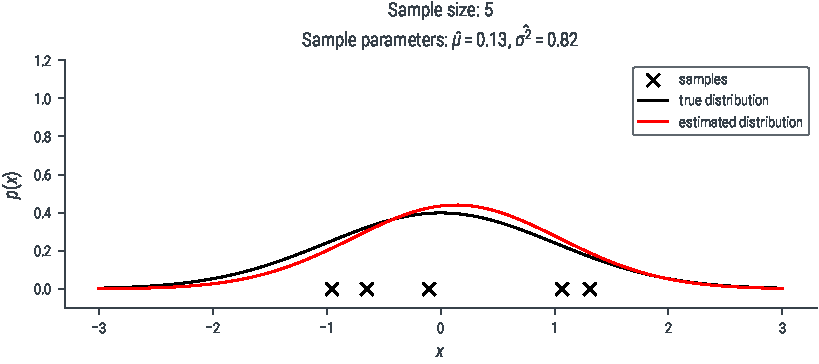
\includegraphics{../figures/mle/biased-mle-normal-5-0.pdf}
            \end{figure}
            
        \end{frame}

             \begin{frame}{Bias }
            \begin{figure}
                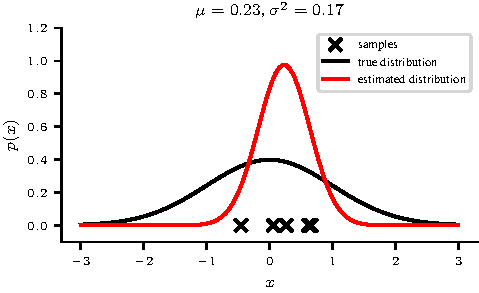
\includegraphics{../figures/mle/biased-mle-normal-5-1.pdf}
            \end{figure}
            
        \end{frame}

             \begin{frame}{Bias }
            \begin{figure}
                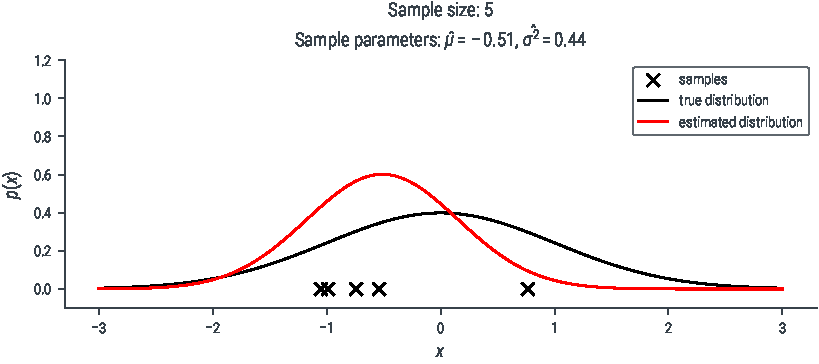
\includegraphics{../figures/mle/biased-mle-normal-5-2.pdf}
            \end{figure}
            
        \end{frame}

             \begin{frame}{Bias }
            \begin{figure}
                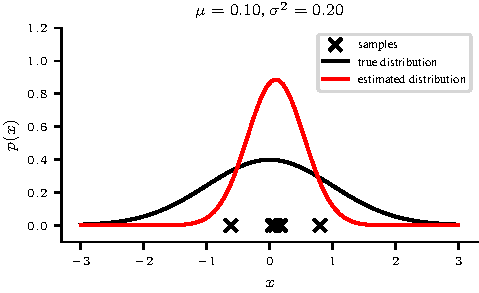
\includegraphics{../figures/mle/biased-mle-normal-5-3.pdf}
            \end{figure}
            
        \end{frame}

             \begin{frame}{Bias }
            \begin{figure}
                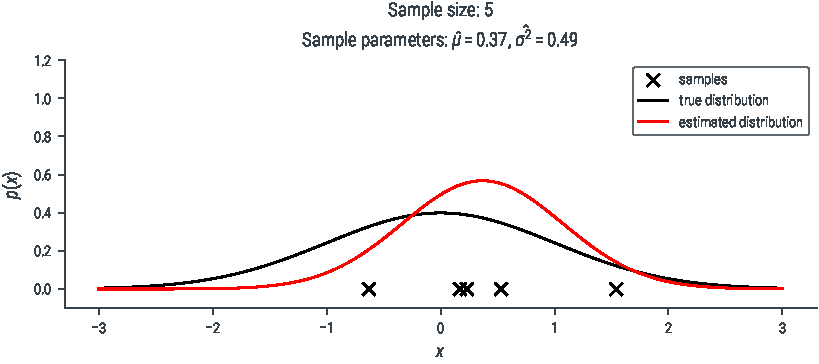
\includegraphics{../figures/mle/biased-mle-normal-5-4.pdf}
            \end{figure}
            
        \end{frame}

             \begin{frame}{Bias }
            \begin{figure}
                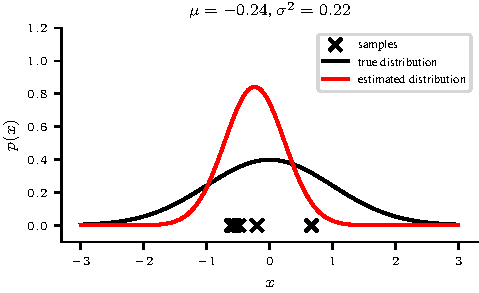
\includegraphics{../figures/mle/biased-mle-normal-5-5.pdf}
            \end{figure}
            
        \end{frame}


    

    


    

\end{document}